\chapter{設計}
\label{chap:third}
%
本章では,使用するQDDモータの説明とロボットアームの基本的な性能や,要求仕様を満たすための設計について述べる.設計には,Autodesk Inventor 2023を使用した.ロボットアームは,6自由度のアームと1軸駆動の平行グリッパで構成されており,前章で述べた要求仕様を満たすように設計されている.アームの主要構成部品は,QDDモータ6基,アルミ板金部品7点,アルミフレーム2本,平行グリッパである.
\begin{figure}[h]
  \centering
  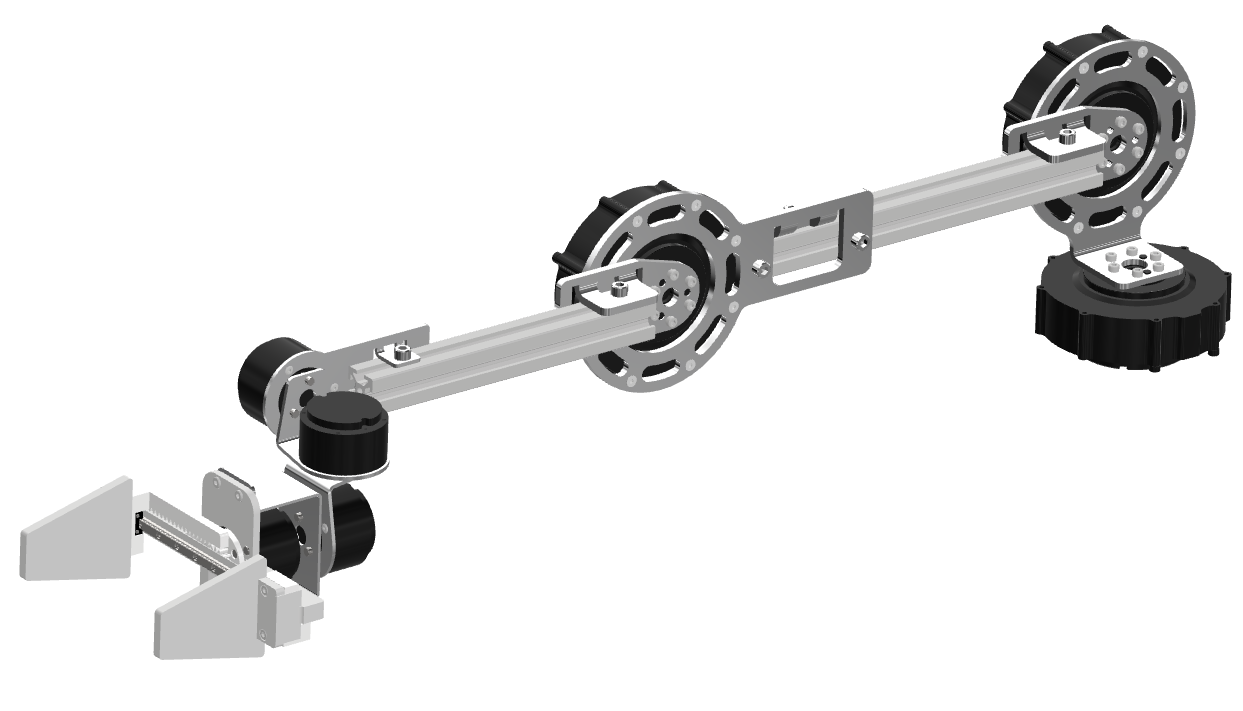
\includegraphics[width=10cm]{images/arm_design.png}
  \caption{Robot arm configuration}
  \label{fig:arm_design}
\end{figure}

%!TEX root = ../thesis.tex
\section{QDDモータの選定}
飯塚ら\cite{飯塚浩太2021}の研究では,減速比10:1のQDDモータが使用されている.また,Zhaoら\cite{10106520}の研究においては,減速比9:1のQDDモータが採用されていた.これらの先行研究は,ロボットアームと人の衝突時の衝撃力軽減を実現するためには,この程度の減速比を持つモータを採用することが有効であることを示唆している.

さらに,本研究ではオープンプラットフォームの観点を重視し,他のロボットアームに使用されているモータと同程度,またはそれ以下の価格であることを選定基準とした.調査対象としたオフィスロボットのうち,ロボットアームに使用しているアクチュエータの価格は,約3万円から約8万円であったため,価格上限を8万円に設定した.

以上を踏まえ,本研究では,持つSteadywinのGIM8108-8とGIM3505-8を採用した.減速比は8:1であり,先行研究で使用されていたモータと同程度の減速比を持つ.また,価格は約19,000円と約18,000円であり,価格上限である8万円を下回っている.
\subsection{選定したモータの性能}
表\ref{tab:QDDComparison}に,選定したQDDモータとReachy\cite{Reachy:online}のアームに使用されているモータ(Dynamixel MX-106T)の比較を示す.選定したSteadywinのGIM8108-8とGIM3505-8は,減速比が8:1で,先行研究で使用していた減速比と近しい物になっている.適切に制御することで衝突時の衝撃を軽減することが可能である.また,許容ラジアル荷重とアキシアル荷重も高いため,追加の補強部品を必要とせずにロボットアームの構造を簡略化することが可能である.
\begin{table}[]
  \centering
  \caption{QDD motor performance comparison}
  \label{tab:QDDComparison}
  \begin{tabular}{lccc}
  \hline
               & \begin{tabular}[c]{@{}c@{}}SteadyWin\\ GIM8108-8\end{tabular} & \begin{tabular}[c]{@{}c@{}}SteadyWin\\ GIM3505-8\end{tabular} & \begin{tabular}[c]{@{}c@{}}Dynamixel\\ MX-106T\end{tabular} \\ \hline
  減速比          & 8 : 1                                                         & 8 : 1                                                         & 225 : 1                                                     \\
  定格トルク(Nm)    & 7.5                                                           & 0.65                                                          & -                                                           \\
  最大トルク(Nm)    & 22                                                            & 1.27                                                          & 10                                                          \\
  重量(g)        & 396                                                           & 97                                                            & 153                                                         \\
  無負荷回転数(rpm)  & 320                                                           & 384                                                           & 55                                                          \\
  許容ラジアル荷重(N)  & 900                                                           & 300                                                           & 40                                                          \\
  許容アキシアル荷重(N) & 225                                                           & 75                                                            & 20                                                          \\
  価格(円)        & 約19,000                                                       & 約18,000                                                       & 約80,000                                                     \\ \hline
  \end{tabular}
\end{table}

\subsection{QDDモータの欠点}
QDDモータは高トルク・高スピードでの動作が可能であるという利点を持つ一方で、この特性は制御が不十分な場合にリスクとなる.特に、通電時に動作が暴走した場合、一般的なモータと比較して周囲の人や機器への被害が大きい.そのため、QDDモータを安全に運用するためには、適切な制御と安全対策が必要である.
\newpage
%!TEX root = ../thesis.tex
\section{基本的な性能}
設計したロボットアームの基本的な性能を述べる.
\subsection{アームサイズ}
図\ref{fig:link_length}にロボットアームのアームリーチとリンク長を示す.人間の腕の長さの比\cite{humanarm:online}を参考に,肩から肘までは290㎜,肘から手首までは220㎜とした.アームリーチは660㎜であり,要求仕様の700㎜程度を満たしている.図\ref{fig:arm_size}にアームサイズを示す.比較のため,机とボトルを模したものを配置している.

\begin{figure}[htbp]
  \centering
  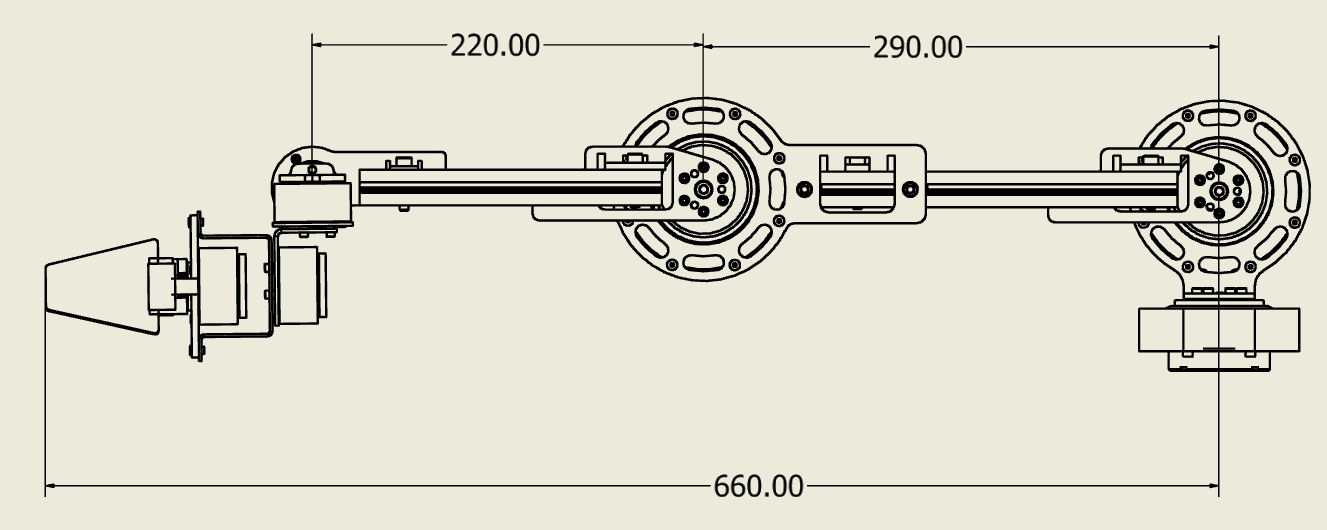
\includegraphics[width=10cm]{images/link_length.png}
  \caption{Arm reach and link length}
  \label{fig:link_length}
\end{figure}

\begin{figure}[htbp]
  \centering
  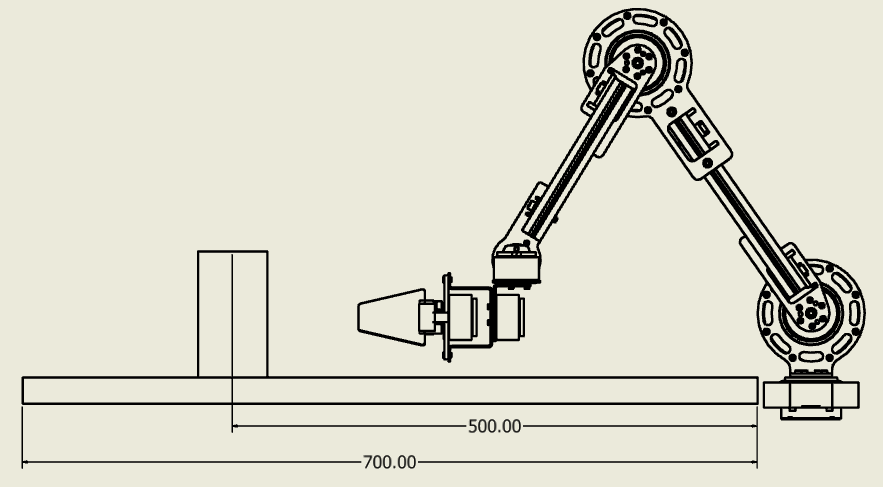
\includegraphics[width=10cm]{images/hikaku.png}
  \caption{Arm size}
  \label{fig:arm_size}
\end{figure}

\clearpage

\subsection{可動範囲}
図\ref{fig:arm_short},図\ref{fig:arm_long}にアームの最小可動範囲と最大可動範囲を示す.最小可動範囲は,アームの部品が干渉することなく動作できる最小の範囲を示しており,最大可動範囲はアームを最大まで伸ばしたときの範囲を示している.

\begin{figure}[htbp]
  \centering
  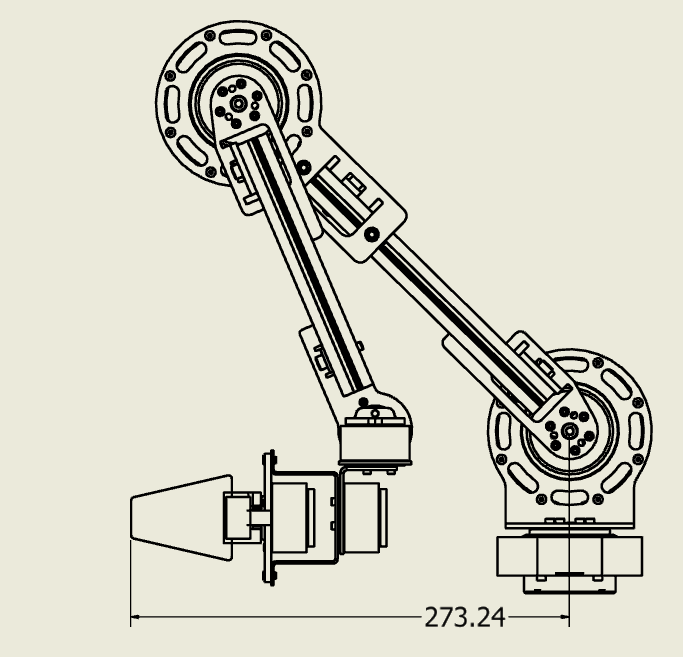
\includegraphics[width=10cm]{images/design/arm_short.png}
  \caption{Minimum range of motion}
  \label{fig:arm_short}
\end{figure}

\begin{figure}[htbp]
  \centering
  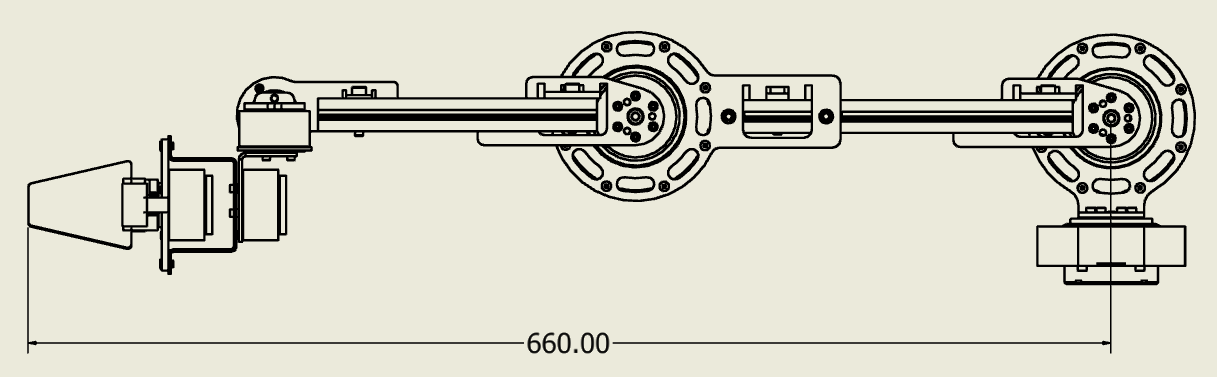
\includegraphics[width=10cm]{images/design/arm_long.png}
  \caption{Minimum range of motion}
  \label{fig:arm_long}
\end{figure}

\subsection{アームの手先の移動}
アームの手先の移動の様子を図\ref{fig:move1},図\ref{fig:move2},図\ref{fig:move3},図\ref{fig:move4}に示す.

\begin{figure}[h]
  \centering
  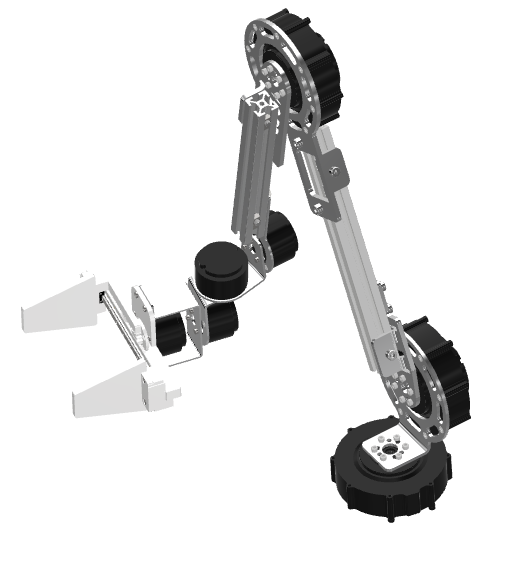
\includegraphics[width=10cm]{images/design/migitika.png}
  \caption{Stretched out to the right}
  \label{fig:move1}
\end{figure}

\begin{figure}[h]
  \centering
  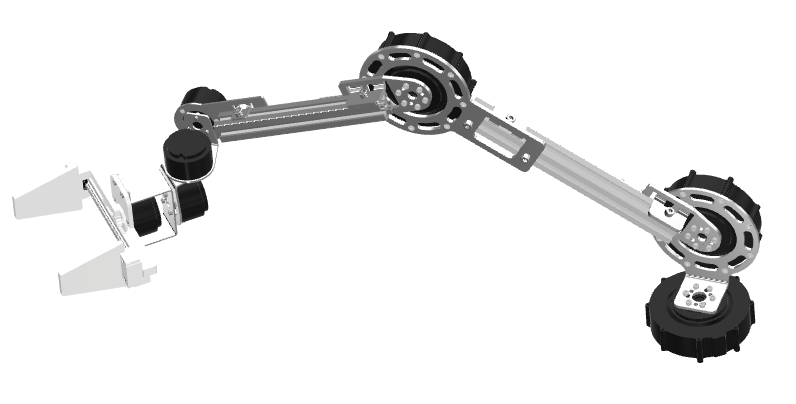
\includegraphics[width=10cm]{images/design/migioku.png}
  \caption{Stretched out to the right}
  \label{fig:move2}
\end{figure}

\begin{figure}[h]
  \centering
  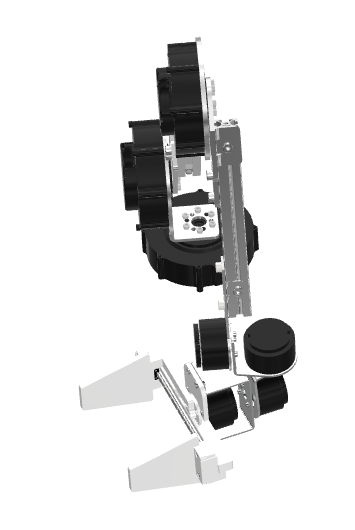
\includegraphics[width=8cm]{images/design/hidaritika.png}
  \caption{Stretched out to the left}
  \label{fig:move3}
\end{figure}

\begin{figure}[h]
  \centering
  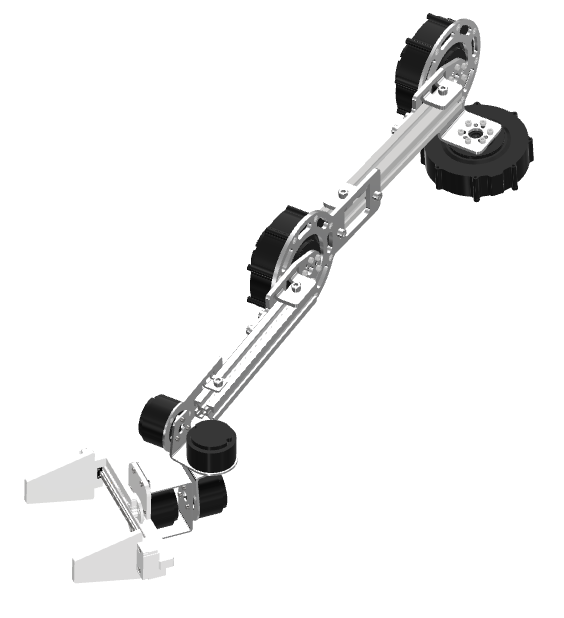
\includegraphics[width=10cm]{images/design/hidarioku.png}
  \caption{Stretched out to the left}
  \label{fig:move4}
\end{figure}
\clearpage

\subsection{可搬重量}
肩ピッチ軸のQDDモータ(SteadyWin GIM8108-8)の定格トルクは7.5Nm,最大トルクは22Nmである.アームを伸ばしたときに自重を支えるために必要なトルクを求め,常時把持することのできる物体の重量と,瞬間的に把持することのできる物体の重量を求める.
\subsubsection{自重を支える為に必要なトルク}
図\ref{fig:CoG}にアームの重心を示す.アームの重心は肩ピッチ軸から0.334mの位置にあり,アームの重さは1.31kgである.重力加速度を9.8m/s$^2$とすると,肩ピッチ軸にかかるトルク$T$は次のように求められる.
\begin{equation}
  T = 1.31 \times 9.8 \times 0.334 = 4.2 Nm
\end{equation}
\begin{figure}[h]
  \centering
  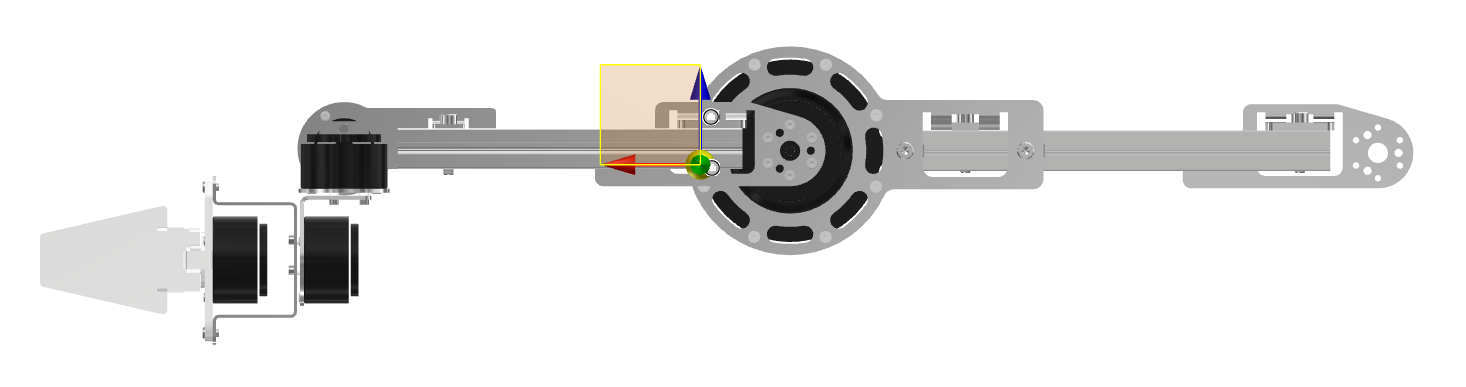
\includegraphics[width=10cm]{images/design/CoG.png}
  \caption{Center of gravity}
  \label{fig:CoG}
\end{figure}

\subsubsection{常時把持することのできる物体の重量}
アームの定格トルクから,自重を支える為に必要なトルクを引くと3.3Nmであり,肩ピッチ軸から手先までの距離は0.66mである.したがって,常時把持することのできる物体の重量$m$は次のように求められる.
\begin{equation}
  m = 3.3 / (9.8 \times 0.66) = 0.51kg
\end{equation}

\subsubsection{瞬間的に把持することのできる物体の重量}
同様に,最大トルクから自重を支える為に必要なトルクを引くと17.8Nmである.したがって,瞬間的に把持することのできる物体の重量$M$は次のように求められる.
\begin{equation}
  m = 17.8 / (9.8 \times 0.66) = 2.75kg
\end{equation}


\clearpage
\newpage
%!TEX root = ../thesis.tex
\section{強度確認}
設計したロボットアームの強度確認のため,Autodesk Inventorの機能である構造解析を行った.解析における安全率が1以上であれば,強度が十分であると判断した.図\ref{fig:shoulder}に肩部の構成を示す.肩部は,ヨー軸モータとピッチ軸モータを繋ぐ図\ref{fig:shoulder}の部品1,およびリンクの一部である,部品2から構成されている.部品1および部品2には,いずれもアルミニウム合金(A5052)を使用している.

本節では,構造解析による部品の強度確認について述べる.

\begin{figure}[h]
  \centering
  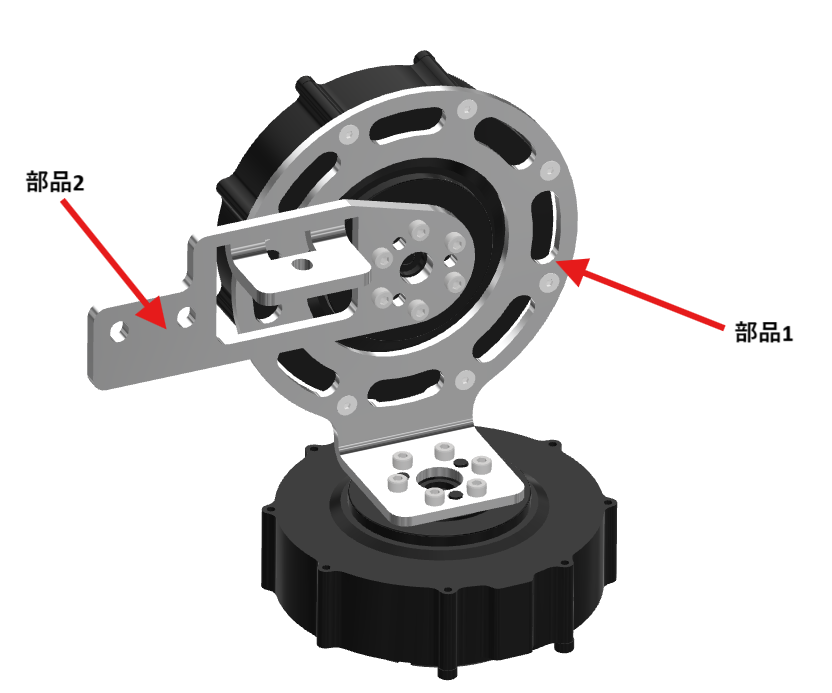
\includegraphics[width=10cm]{images/design/shoulder.png}
  \caption{Configuration of the shoulder components}
  \label{fig:shoulder}
\end{figure}

\subsection{部品1の構造解析}
図\ref{fig:shoulder}の部品1は,ヨー軸モータが最大出力22Nmを発生した際に最大負荷を受ける部品である.図\ref{fig:T3_40}に構造解析結果を示し,設計仕様を表\ref{tab:part1_spec}にまとめた.解析の結果,安全率は0.39であり,強度が不足していることが確認された.特に,図\ref{fig:T3_40}の結果から,曲げ加工部分において強度が不足していることが明らかとなった.この課題を解決するため,「板厚を変更した部品」と「形状を変更した部品」の2つの設計案を検討し,それぞれ再解析を実施した.

\begin{figure}[h]
  \centering
  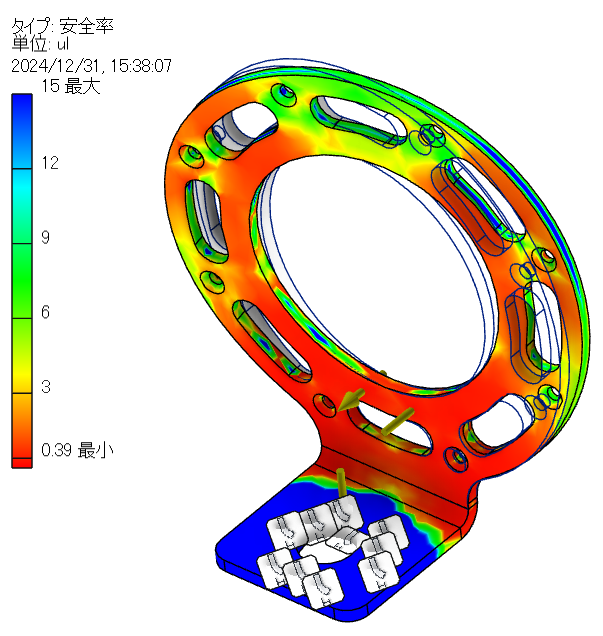
\includegraphics[width=6cm]{images/design/T3_40.png}
  \caption{Structural analysis results of Part 1}
  \label{fig:T3_40}
\end{figure}

\begin{table}[h]
  \centering
  \caption{Specifications of Part 1}
  \begin{tabular}{lc}
    \hline
    厚み & 3㎜ \\ 
    質量 & 43.6g \\ 
    安全率 & 0.39 \\ \hline
  \end{tabular}
  \label{tab:part1_spec}
\end{table}
\clearpage

\subsection{設計の変更}
部品の形状はそのままに,板厚を3mmから5mmに変更した場合の構造解析結果を図\ref{fig:T5}に示し,設計仕様を表\ref{tab:part1_spec_T5}にまとめた.解析の結果,安全率は基準の1を超え,強度が十分であることが確認された.ただし,質量が27.5g増加するという結果が得られた.

\begin{figure}[h]
  \centering
  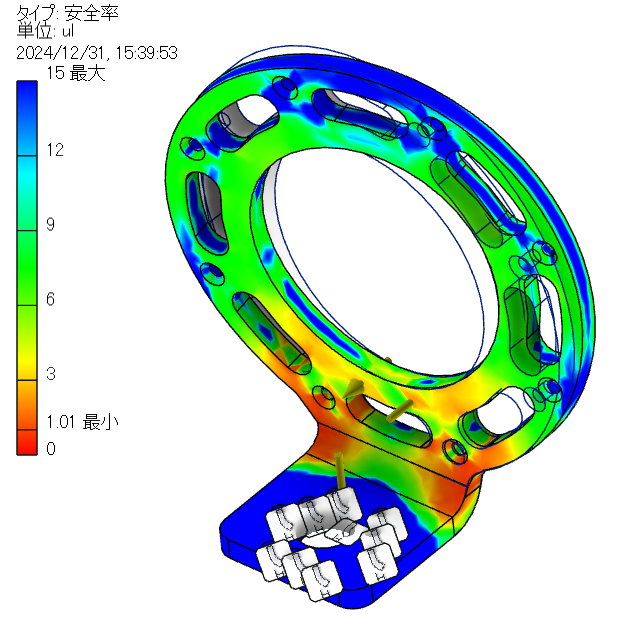
\includegraphics[width=6cm]{images/design/T5.png}
  \caption{Structural analysis results of Part 1 (thickness changed to 5mm)}
  \label{fig:T5}
\end{figure}

\begin{table}[h]
  \centering
  \caption{Specifications of Part 1 (thickness changed to 5mm)}
  \begin{tabular}{lc}
    \hline
    厚み & 5㎜ \\ 
    質量 & 71.1g \\ 
    安全率 & 1.01 \\ \hline
  \end{tabular}
  \label{tab:part1_spec_T5}
\end{table}
\clearpage

次に,板厚を変更せず,形状の改良を行った場合の解析結果を図\ref{fig:T3_80}に示し,設計仕様を表\ref{tab:part1_spec_T3_80}にまとめた.具体的には,図\ref{fig:T3_40}の解析結果を基に,特に強度が不足していると判明した曲げ加工部分の幅を広げる設計変更を行った.

解析の結果,安全率が基準を満たし,十分な強度を確保できることが確認された.また,重量は61.8gであり,板厚を変更した場合(表\ref{tab:part1_spec_T5}参照)と比較して軽量化を実現した.

以上の解析結果を踏まえ,図\ref{fig:shoulder}の部品1について,曲げ加工部分の幅を広げた設計変更を最終設計として採用した.

\begin{figure}[h]
  \centering
  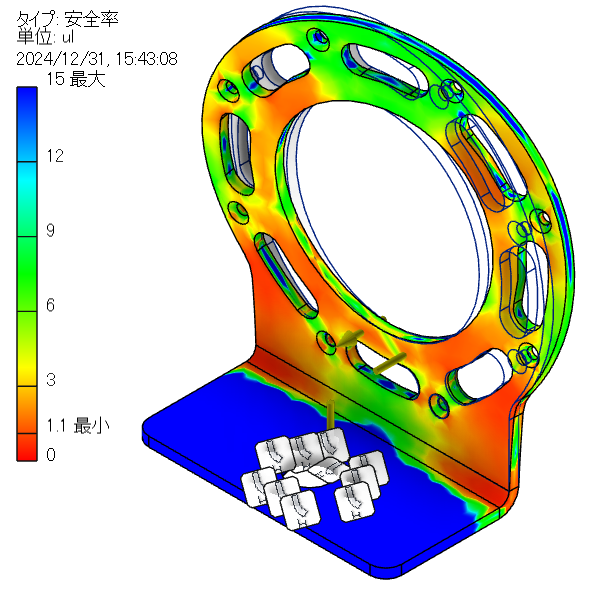
\includegraphics[width=6cm]{images/design/T3_80.png}
  \caption{Structural analysis results of Part 1 (shape optimized)}
  \label{fig:T3_80}
\end{figure}

\begin{table}[h]
  \centering
  \caption{Specifications of Part 1 (shape optimized)}
  \begin{tabular}{lc}
    \hline
    厚み & 3㎜ \\ 
    質量 & 61.8g \\ 
    安全率 & 1.1 \\ \hline
  \end{tabular}
  \label{tab:part1_spec_T3_80}
\end{table}

\subsection{部品2の構造解析}
図\ref{fig:shoulder}の部品2は,アルミフレームを2方向から固定する形状を採用している(図\ref{fig:pitchalumi}参照).最大負荷条件(22Nm)の下で構造解析を実施した結果を図\ref{fig:pitch}に示す.現行の設計では,安全率が0.47と低く,特に赤色で示された箇所において強度不足が確認された.

\begin{figure}[h]
  \centering
  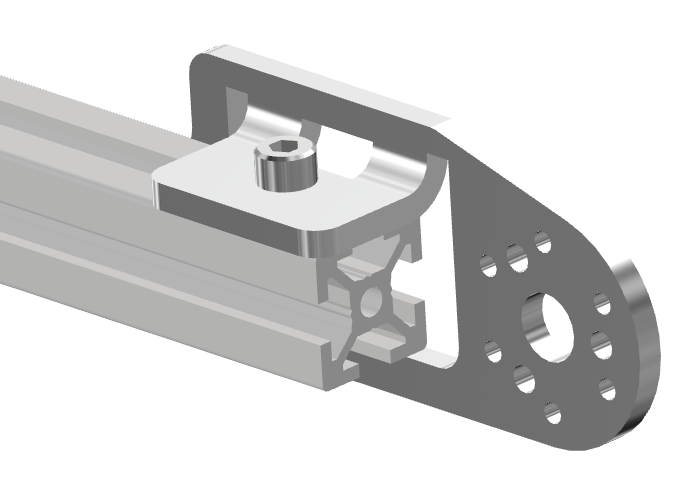
\includegraphics[width=6cm]{images/design/pitchlink.png}
  \caption{Fixing the aluminum frame and part 2}
  \label{fig:pitchalumi}
\end{figure}

\begin{figure}[h]
  \centering
  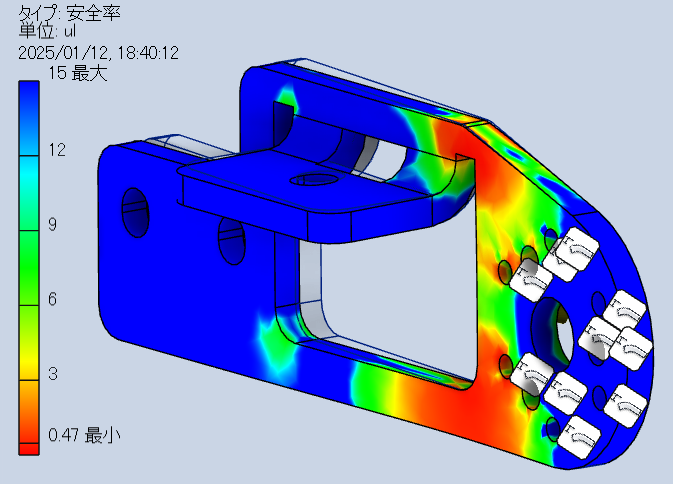
\includegraphics[width=6cm]{images/design/pitch.png}
  \caption{Structural analysis results of Part 2 at maximum output of 22Nm}
  \label{fig:pitch}
\end{figure}

部品の厚みを5mmに変更した場合,安全率は0.58に改善したものの,依然として基準に満たなかった.このため,定格出力(7.5Nm)の条件下で再解析を実施した.解析結果を図\ref{fig:pitchok}に示し,設計仕様を表\ref{tab:part2_spec}にまとめた.この結果,定格条件下では安全率が基準を満たし,十分な強度を確保できることが確認された.

以上より,現設計において部品2の形状変更は行わないこととし,最大出力時の安全率の確保を今後の課題とする.
\begin{figure}[h]
  \centering
  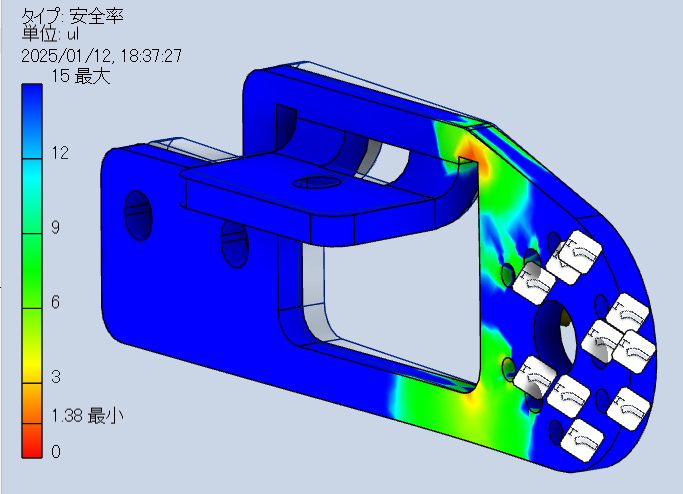
\includegraphics[width=6cm]{images/design/pitchok.png}
  \caption{Structural analysis results of Part 2 at rated output 7.5Nm}
  \label{fig:pitchok}
\end{figure}
\begin{table}[h]
  \centering
  \caption{Specifications of Part 2}
  \begin{tabular}{lc}
    \hline
    厚み & 5㎜ \\ 
    質量 & 34.0g \\ 
    安全率 & 1.38 \\ \hline
  \end{tabular}
  \label{tab:part2_spec}
\end{table}

\newpage
%!TEX root = ../thesis.tex
\section{平行グリッパの設計}
本研究では,リニアガイドとラック&ピニオン機構を用いた平行グリッパを設計した.図\ref{fig:hand}は平行グリッパの分解図である.グリッパの開閉には,QDDモータ(Steadywin GIM3505-8)を使用し,モータに取り付けたギアを介してラック&ピニオン機構で駆動する.グリッパのスライド部分にはリニアガイドを採用している.また,黄色の部品は3Dプリンタでの製作を行う.
\begin{figure}[htbp]
  \centering
  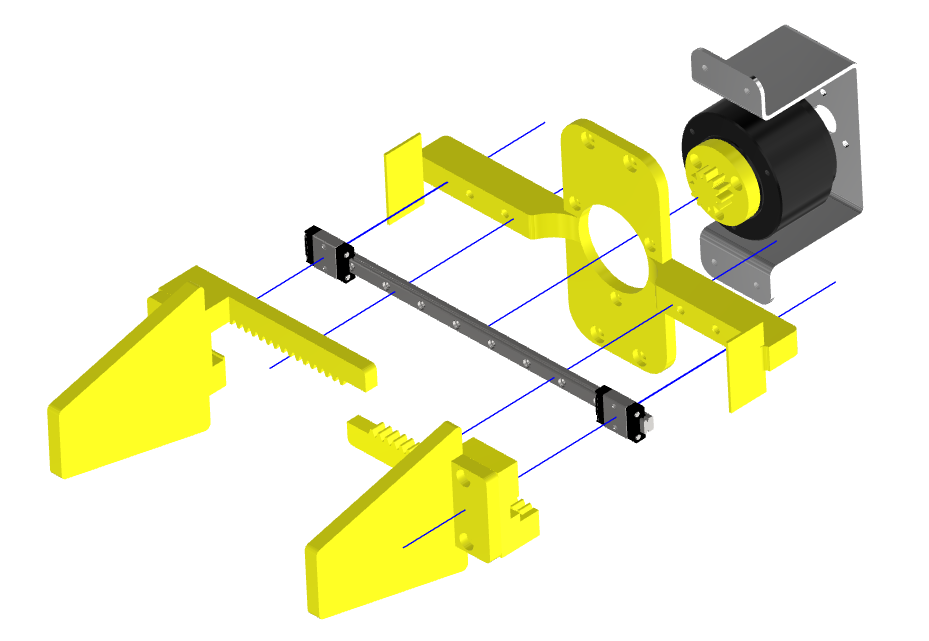
\includegraphics[width=10cm]{images/design/hand.png}
  \caption{Exploded view of parallel gripper}
  \label{fig:hand}
\end{figure}

\newpage
%